\chapter{The SANA Experiments}
\label{sec:sana}

Power densities of gas-cooled \glspl{pbr} are typically low enough that radiation and conduction between touching pebbles, in combination with an ex-vessel water cooling system, is sufficient to remove decay heat in a depressurized \gls{lofc} by natural convection cooling. However, low power densities result in larger reactor vessels that both complicate rail transport and increase structural material costs. Economic feasibility may motivate stretching paper design concepts to higher power densities or uprating an existing reactor. Safe reactor operation requires \gls{th} models that can accurately model natural convection decay heat removal and the proximity of fuel temperatures to maximum allowable operating limits, especially when maximization of power density is a primary design objective. 

% TODO: put this in the introduction section when describing the motivation for this section
%Validation of a computational model for conduction cool-down conditions is necessary to establish additional margins associated with the predictive nature of modeling tools for decay heat removal.

The SANA facility is a scaled experiment built and operated in Germany in the mid 1990s that models depressurized cool-down of gas-cooled \glspl{pbr} as a function of power density, coolant, and pebble properties \cite{SANA}. This section presents Pronghorn simulations of all steady-state and axisymmetric SANA experiments to assess the capability of the macroscale model for predicting core temperatures in depressurized \gls{lofc} events. This validation exercise is one piece of a much larger test matrix designed to qualify the multiscale model and its implementation in Pronghorn for gas- and liquid-cooled \glspl{pbr} \cite{ph_plan}.

The accuracy of porous media simulations is dependent on the closure relationships used to describe the solid-fluid phase distribution, interphase momentum and energy transfer, and lumped parameter effective heat transfer. Few \gls{th} simulations of reactor conditions have quantified the sensitivity of temperature predictions to the selection of particular closures from the enormous literature on the subject. For instance, a distillation of this literature over the course of a five year PhD project has resulted in the implementation of seven porosity models; four friction factor models; five interphase convective heat transfer coefficient models; 245 effective solid conductivity models as permutations of the seven \(\kappa_\text{radiation}\) models, seven \(\kappa_\text{conduction}\) models, and five \(\kappa_\text{contact}\) models; and two effective fluid conductivity models. The selection of these particular correlations for implementation in Pronghorn reflects their prominence in the porous media literature, and is by no means exhaustive. 

Due to the wealth of solid temperature data available, the SANA experiments are a useful baseline data set from which the sensitivity of pebble temperatures to variations in macroscale model closures can be obtained. By individually varying the porosity, near-wall effective solid thermal conductivity, interphase heat transfer and drag, and thermal dispersion models\mdash the five closures that tend to vary the most between applications of the macroscale model in Chapter \ref{sec:PhysicalModels} to gas-cooled \glspl{pbr}\mdash guidelines for closure selection and development are provided.

The remainder of this section is organized as follows. Section \ref{sec:experimental} introduces the SANA facility and experiments. Section \ref{sec:model} describes the Pronghorn model of the facility. Section \ref{sec:baseline} then presents simulation results for all 52 of the steady-state and axisymmetric experiments performed, plus an open upper plenum case, using a single set of baseline macroscale closures. When available, code-to-code comparisons are made to Flownex and GAMMA, two porous media applications that have previously been used to model gas-cooled \glspl{pbr} \cite{duToit2006,lim}. Simulation data has graciously been provided by Dr. C. G. Du Toit of the School of Mechanical and Nuclear Engineering at North-West University, South Africa and Dr. H. S. Lim of \gls{kaeri}.

In Section \ref{sec:sensitivity}, macroscale closures are individually varied from the baseline set used in Section \ref{sec:baseline} to determine the sensitivity of pebble temperature to closure selection. Finally, Section \ref{sec:5_summary} provides conclusions on the applicability of the friction-dominated macroscale model to the simulation of depressurized conduction cool-down in gas-cooled \glspl{pbr}, with particular emphasis on the importance of closure selection in future modeling activities and recommendations for experimental programs aimed at new closure development.

\section{The SANA Facility}
\label{sec:experimental}

The SANA facility consists of a cylindrical steel vessel containing about 9500 non-fueled pebbles heated by electrical resistance heaters in a variety of configurations in both steady and transient conditions \cite{SANA}. A depiction of the facility in a full-length, single-heater configuration is shown in Fig.\ \ref{fig:SANA_core}. Insulation on the bottom and top of the bed limits axial heat loss. The pebble surface temperature is measured throughout the bed with thermocouples at five different elevations, indicated as ``bottom,'' ``near bottom,'' ``middle,'' ``near top,'' and ``top'' in Fig.\ \ref{fig:SANA_core}. The precise axial coordinate of these measurement planes varied from test to test, and the scale shown in Fig.\ \ref{fig:SANA_core} is approximate. Most experiments involved a single centrally-located heater in an axisymmetric configuration, though several experiments placed multiple heaters throughout the bed so that the power distribution was no longer axisymmetric; these cases are not considered here.

\begin{figure}[h!]
\centering
\hspace{1.3cm}
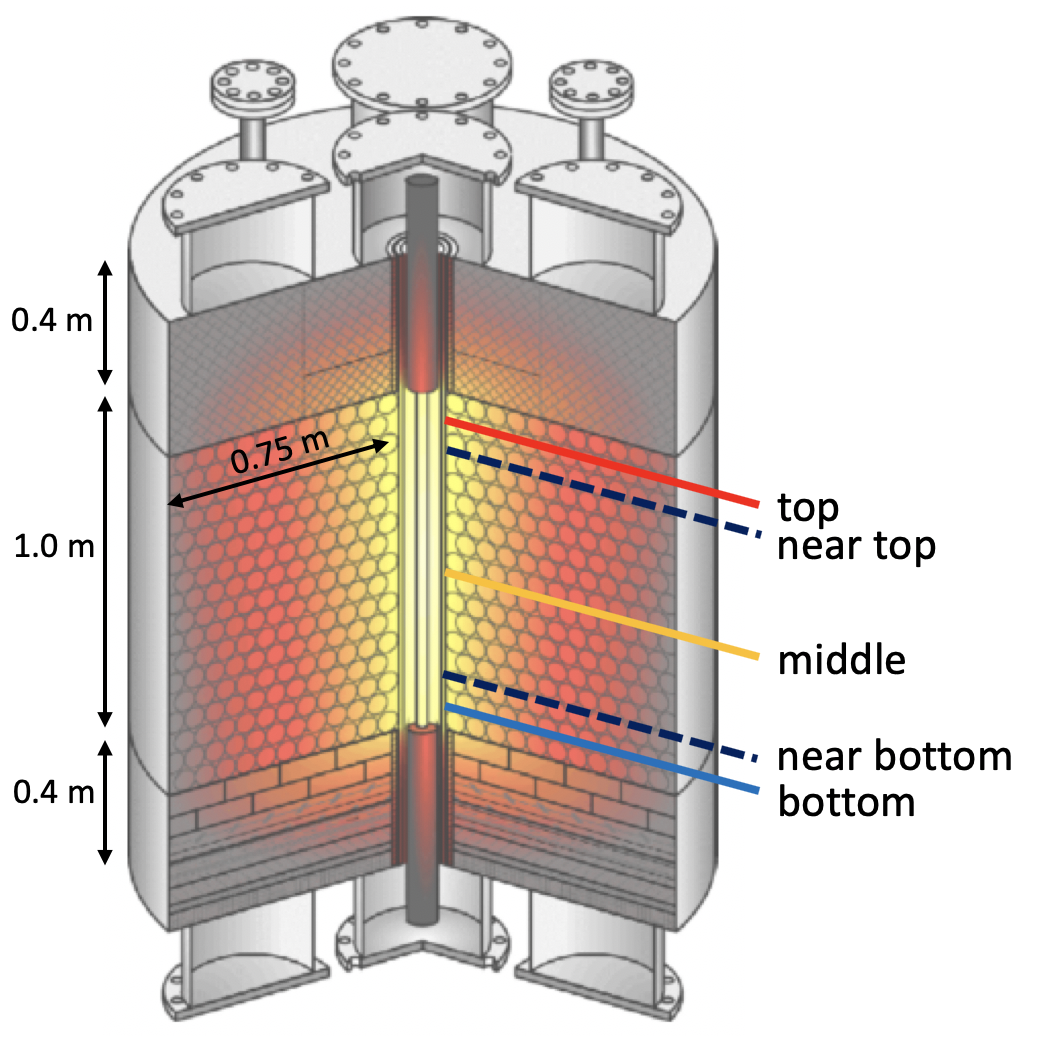
\includegraphics[width=0.5\linewidth]{figs/sana_core_labeled.png}
\caption{Illustration of the SANA facility with a single full-height heater. Temperature measurement planes are indicated as ``bottom,'' ``near bottom,'' ``middle,'' ``near top,'' and ``top'' (adapted from \cite{SANA}).}
\label{fig:SANA_core}
\end{figure}

A total of 52 steady-state and axisymmetric experiments were conducted with three different pebble designs, two different coolants, four different heater configurations, and seven different heater powers, resulting in a total of nearly 1300 solid temperature measurements. Fig.\ \ref{fig:sana_permutation} shows these experimental settings that, when permuted, encompass all the settings of the 52 experiments. Some heater configurations were only performed with 6 \si{\centi\meter} graphite pebbles, so not all experiments implied by Fig.\ \ref{fig:sana_permutation} were necessarily conducted, though all settings are represented.

The three pebble designs\mdash 6.5 \si{\centi\meter} diameter aluminum oxide, 6 \si{\centi\meter} diameter electric graphite, and 3 \si{\centi\meter} matrix graphite\mdash vary in their diameter and thermal properties. The smaller the pebble diameter, the greater the interphase friction and convective heat transfer. The three pebbles also have significantly different thermal conductivities; the electric graphite thermal conductivity is approximately two times and ten times larger than that of the matrix graphite and aluminum oxide, respectively. The higher the pebble thermal conductivity, the greater the effective solid thermal conductivity and heat transfer mechanisms independent of convection.

\begin{figure}[!h]
\centering
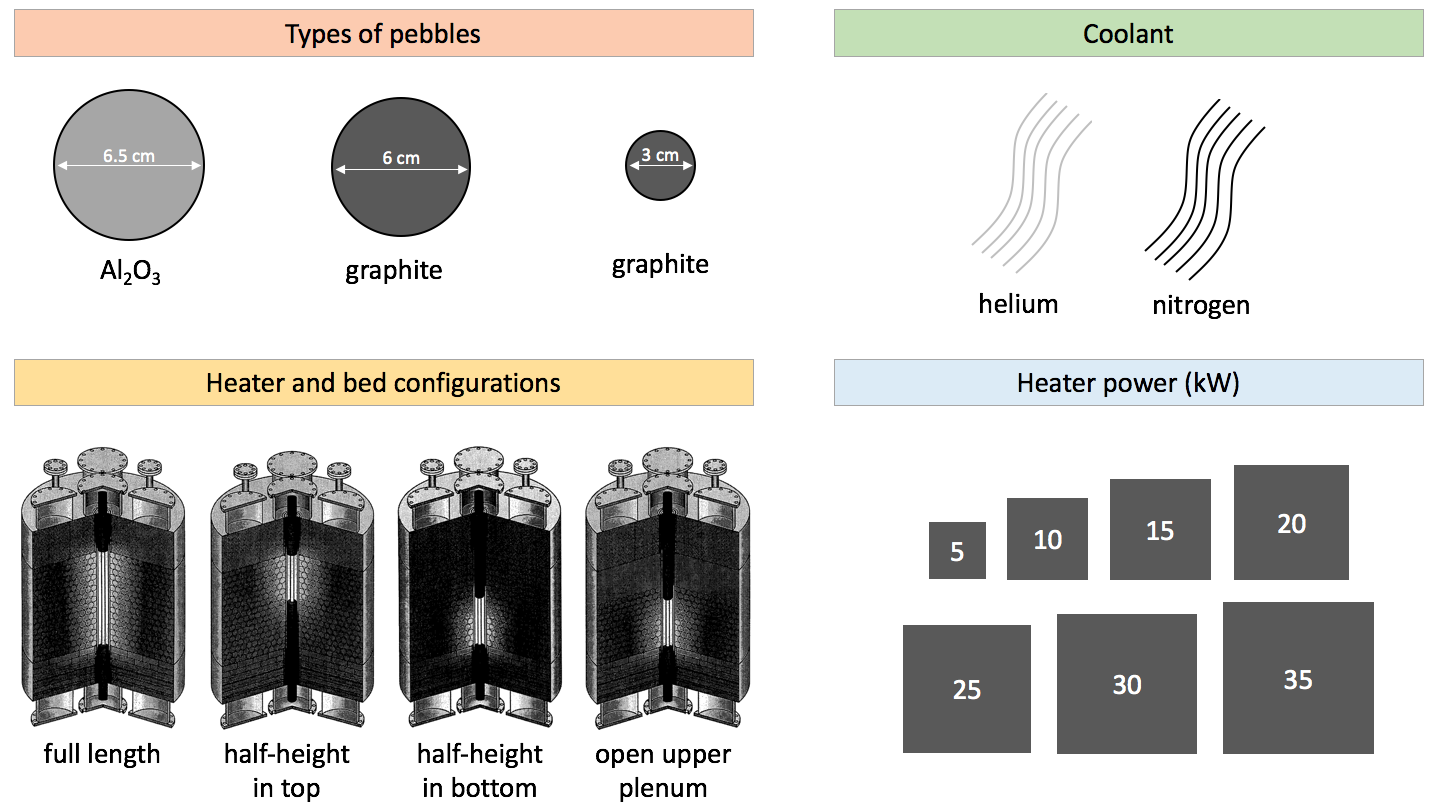
\includegraphics[width=0.9\linewidth]{figs/sana_permutation.png}
\caption{Experimental matrix for the 52 steady-state and axisymmetric SANA experiments (adapted from \cite{SANA}).}
\label{fig:sana_permutation}
\end{figure}

Experiments are performed with both helium and nitrogen due to the extensive use of helium coolant and nitrogen's thermodynamic similarity to air, barring high graphite corrosion rates. The SANA facility operates at atmospheric pressure, so both coolants correspond to depressurized \gls{lofc} conditions; experiments with nitrogen represent surrogates for air ingress, where natural convection cooling is distinct from that with helium. Helium and nitrogen have significantly different thermal properties; the helium thermal conductivity is approximately five times larger than that of nitrogen, resulting in stronger convective transport but weaker diffusive transport in nitrogen than in helium. The various combinations of pebble design and coolant result in different relative strengths of convective to diffusive transport and buoyant forces to friction losses. 

The partial length heater configurations are surrogates for partial control rod insertion, while the open plenum case models the bed-cavity interface found in most gas-cooled \glspl{pbr}. Finally, the various heater powers correspond to the decreasing decay heat levels at various times following an initial shutdown. The maximum power density of 28 \si{\kilo\watt\per\cubic\meter} corresponds to about 1\% of the full power of a typical gas-cooled \gls{pbr} design, or decay heat levels several hours after shutdown.

All 52 of the steady-state and axisymmetric cases are simulated with Pronghorn. Validation results for eight cases are presented in detail, while the remaining 44 are summarized with error histogram plots. These eight cases are selected to cover most of the range of powers, heater arrangements, coolants, and pebble types used in the experiments, in addition to permitting direct comparison with the available Flownex and GAMMA results. Fluid temperature and velocity results, for which no experimental data was collected, are also shown for a number of additional experiments aside from the eight highlighted cases. Table \ref{table:CasesLetters} summarizes these eight cases and provides case letters for differentiation. One experiment with an open upper plenum is discussed as a separate demonstration of the macroscale model's capabilities for predicting bed-to-plenum heat and mass transfer.

\begin{table}[h!]
\caption{A summary of the SANA cases simulated with Pronghorn and presented in detail in this text. Case letters are provided for reference.}
\centering
\begin{tabular}{|c|c|c|c c c|}
\hline\hline
Case & Heater description & Pebble Type & \(d_p\) (\si{\centi\meter}) & Fluid & Power (\si{\kilo\watt})\Tstrut\Bstrut\\
\hline
A & full-height & graphite & 6.0 & He & \color{white}0\color{black}5\Tstrut\\
B & full-height & graphite & 6.0 &He & 35\\
C & full-height & graphite & 6.0 & N & \color{white}0\color{black}5\\
D & full-height & graphite & 6.0 & N & 35\Bstrut\\
\hline
E & full-height & aluminum oxide & 6.5 & He & 30\Tstrut\\
F & full-height & aluminum oxide & 6.5 & N & 30\Bstrut\\
\hline
G & bottom half & graphite & 6.0 & He & 20\Tstrut\\
H & bottom half & graphite & 6.0 & N & 20\Bstrut\\
\hline
I & bottom half, open plenum & graphite & 6.0 & N & \color{white}0\color{black}5\Tstrut\Bstrut\\
\hline
\end{tabular}
\label{table:CasesLetters}
\end{table}

\section{Computational Model}
\label{sec:model}

The low power and absence of forced convection cooling results in slow natural circulation flows with momentum conservation dominated by drag effects. Therefore, the friction-dominated model in Eq. \eqref{eq:PrimitiveEqns} is used for the macro length scale. The homogeneous pebble interiors and steady-state conditions preclude the need for mesoscale and microscale models because the temperature everywhere in a pebble with no heat source is equal to its uniform surface temperature. Helium and nitrogen properties are obtained with the \gls{sbtl} method described in Appendix \ref{sec:props}. Pebble properties are given in Appendix \ref{sec:props}.

The lack of significant azimuthal asymmetries justifies the use of a 2-D cylindrically-symmetric geometry. For simplicity, only the interior of the vessel is modeled. That is, the left boundary coincides with the heater surface, the right boundary coincides with the inner surface of the vessel, and the bottom and top boundaries coincide with the inner surfaces of the insulation. The effects of the vessel and insulation on heat transfer are approximated using the thermal resistance concept\mdash the heat flux on a boundary is modeled as series conduction through a number of homogeneous layers, followed by parallel convection and radiation from the vessel surface to the ambient. That is, the boundary heat flux \(\tilde{q}\) is approximated as

\begin{equation}
\label{eq:ThermalResistanceBC}
\tilde{q}=\frac{T-T_\infty}{A_b\left\lbrack\sum_{i\ =\ 1}^{n_l}R_{\text{cond},i}+\frac{1}{\left(h_c+h_r\right)A_s}\right\rbrack}\ ,
\end{equation}

\noindent where \(A_b\) is the area of the boundary; \(A_s\) is the area of the surface; \(n_l\) is the number of conduction layers; \(R_{\text{cond},i}\) is the conduction resistance of the \(i\)-th layer; \(h_c\) is the convective heat transfer coefficient; and \(h_r\) is the radiation heat transfer coefficient,

\begin{equation}
\label{eq:RadiationHTC}
h_r=\varepsilon\sigma\left(T_\text{surf}^2+T_\infty^2\right)\left(T_\text{surf}^{\color{white}1\color{black}}+T_\infty\right)\ ,
\end{equation}

\noindent where \(T_\text{surf}\) is the surface temperature. In Eqs. \eqref{eq:ThermalResistanceBC} and \eqref{eq:RadiationHTC}, ``boundary'' refers to the mesh sideset where the \gls{bc} is applied and ``surface'' refers to the interface between the \(n_l\)-th conduction layer and the ambient. An under-relaxed fixed point iteration is performed to obtain \(T_\text{surf}\). Eq. \eqref{eq:ThermalResistanceBC} approximates the heat transfer through the conduction layers as unidirectional along \(\hat{n}\) and may not be accurate for very large thermal gradients in directions parallel to \(\hat{n}\).

On the bottom, top, and right boundaries, the heat flux applied to the solid energy conservation equation is given by Eq. \eqref{eq:ThermalResistanceBC} with constant insulation and vessel thermal properties \cite{SANA}. The vessel emissivity and convection heat transfer coefficient are assumed to be 0.8 and 15 \si{\watt\per\square\meter\per\kelvin}, respectively. Neither of these values are provided with the benchmark documentation, so both values were selected to be in the center of the ranges used by other participants \cite{rousseau,baggemann,becker2003,lim,tecdoc1163}. Due to the lower thermal conductivity of the fluid phase and the low velocities expected, the fluid is assumed insulated on the bottom, top, and right boundaries.

On the heater surface, the total heat flux \(\tilde{q}_\text{tot}\) is assumed uniform and is split between the phases according to the effective thermal conductivities \cite{alazmi}. On the left boundary, the heat flux into the solid phase is given as

\begin{equation}
\label{eq:HeatFluxSplitting}
\tilde{q}=\frac{\kappa_s}{\kappa_f+\kappa_s} \tilde{q}_\text{tot}\ ,
\end{equation}

\noindent while the heat flux into the fluid phase comprises the remainder of the total heat flux. Eq. \eqref{eq:HeatFluxSplitting} is a very crude approximation of the multi-phase heat transfer processes that occur near walls in packed beds. Other simplified \glspl{bc} have been proposed \cite{alazmi}, but preliminary tests with different \glspl{bc} did not show any clear advantage of any one option over another. Finally, zero normal mass flux is weakly imposed on all surfaces, while tangential slip is permitted. 

The baseline set of macroscale closures used in Section \ref{sec:baseline} are as follows. The friction factor is given by Eq. \eqref{eq:W_KTA}, the interphase heat transfer coefficient is given by Eq. \eqref{eq:KTA}, and the effective fluid thermal conductivity is given by Eq. \eqref{eq:KappaFluidBasic}. The effective solid thermal conductivity is given by the sum of Eqs. \eqref{eq:KappaRadiationBB}, \eqref{eq:KappaFluidConductionZS}, and \eqref{eq:KappaSolidConductionCT}, with Eq. \eqref{eq:Tsotsas} applied within a half pebble diameter of the walls as a correction to \(\kappa_\text{radiation}\). For all three pebble types, the emissivity, elastic modulus, and Poisson ratio are assumed to be 0.8, \(9\times10^9\) Pa, and 0.136, respectively\mdash values typically ascribed to \gls{pbr} fuel pebbles\mdash since more detailed information was not available. 

No information is available regarding the bed filling method, so \(\epsilon_\infty\) is selected as 0.39, a value commonly used for packed sphere beds. For all cases except the open plenum case, the porosity is given by Eq. \eqref{eq:ExpPorosity2} with \(\epsilon_\text{wall}=0.8\). For the open plenum case, the porosity in the plenum is unity and in the bed is given by Eq. \eqref{eq:ExpPorosity2} with \(\epsilon_\text{wall}=1\) to ensure a smooth transition to the plenum in the near-wall region.

All cases are run as pseudo-transients, terminating once the relative change in the solution norm from the previous time step is less than \(10^{-6}\). Mesh refinement studies are performed for the highest-powered cases of each experiment category (such as nitrogen coolant with 3 \si{\centi\meter} pebbles and a long central heater) to ensure converged results, but for brevity are not shown here. 

To enable reproduction of the simulations presented in this chapter, Appendix \ref{sec:reproducibility} lists all data and input files related to this chapter.

\section{Baseline Results}
\label{sec:baseline}

This section presents Pronghorn simulations for the 52 steady-state and axisymmetric SANA experiments and one open plenum test using the baseline set of closures described at the end of Section \ref{sec:model}. 

Section \ref{sec:sana_subset} presents detailed validation results for the select cases given in Table \ref{table:CasesLetters}. All 52 steady-state and axisymmetric cases are summarized in Section \ref{sec:AllTests}. To avoid repeating the same error discussion with each new validation case, all discussion of the effects of modeling simplifications and differences in the Pronghorn, Flownex, and GAMMA models is deferred to Section \ref{sec:AllTests}.

\subsection{A Selected Subset of the Experiments}
\label{sec:sana_subset}

A total of nearly 1300 solid temperature measurements were made across the steady-state and axisymmetric SANA experiments. While no fluid temperature or velocity data was recorded, a qualitative discussion of the effect of coolant and pebble properties on flow and heat transport provides useful physical intuition for understanding the solid temperature data. Fig.\ \ref{fig:streamlines2} shows Pronghorn predictions of fluid temperature and velocity streamlines for the six experiments with a long central heater and 30 \si{\kilo\watt} heater power. The top and bottom rows show predictions for helium and nitrogen coolant, respectively. The left, middle, and right columns show predictions for 6 \si{\centi\meter} electric graphite pebbles, 3 \si{\centi\meter} matrix graphite pebbles, and 6.5 \si{\centi\meter} aluminum oxide pebbles, respectively. In each figure, the left axis is adjacent to the heater and represents the $r$-$z$ symmetry axis. 

A natural convection flow is established as fluid buoyantly rises near the heater surface and cools near the vessel outer surface. The insulation on the bottom and top of the bed induces primarily radial temperature gradients. The low thermal conductivity of nitrogen results in more significant convective transport than in helium, which manifests as larger axial fluid temperature gradients and a recirculation vortex located closer to the bottom of the bed. The thermal conductivity of the pebbles is directly related to the maximum temperature in the bed\mdash from left to right, the pebble thermal conductivity decreases. Experiments with aluminum oxide pebbles and nitrogen coolant have the greatest convective heat transport, while experiments with 6 \si{\centi\meter} graphite pebbles and helium coolant have the greatest diffusive heat transport. 

Moving to the solid temperature predictions, similar trends in the solid temperature with pebble and coolant thermal properties will be highlighted with each case. In presenting the validation data, all experimental results are shown as discrete points and Pronghorn predictions are shown as solid lines (---). When available, Flownex results are shown as dashed lines (- -) and GAMMA results are shown as dotted lines ($\cdots$). Measurements were taken at the five axial elevations shown in Fig.\ \ref{fig:SANA_core}, but only three of these elevations are plotted to simplify data presentation.

\begin{figure}[h!]
\centering
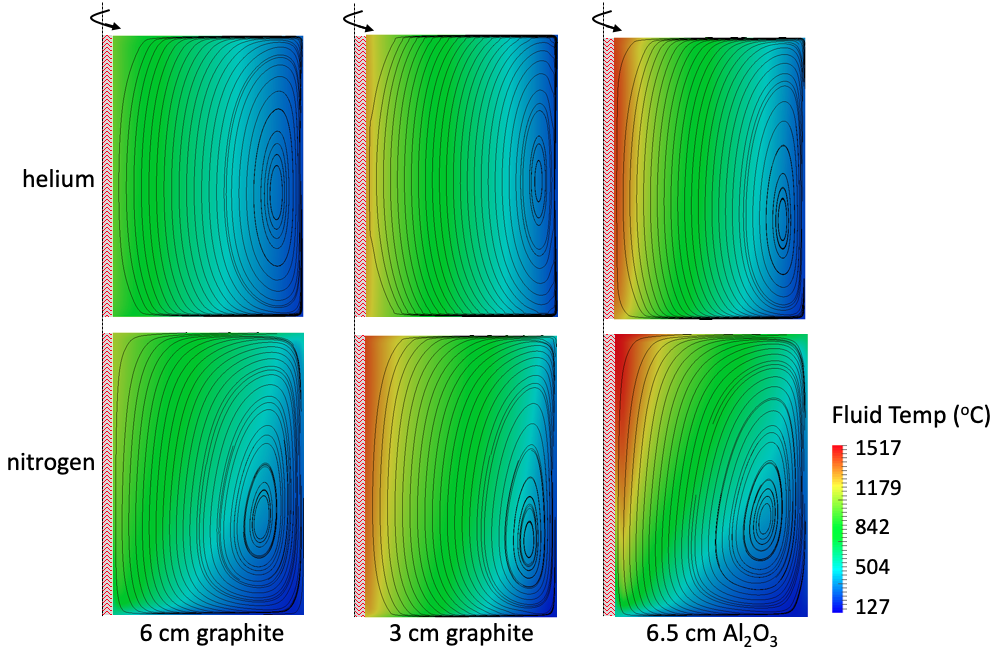
\includegraphics[height=0.65\linewidth]{figs/sana_30kW_vel.png}
\caption{Pronghorn predicted fluid temperature and velocity streamlines for a 30 \si{\kilo\watt} heater power for helium (top row) and nitrogen (bottom row) coolant for the three pebble types.}
\label{fig:streamlines2}
\end{figure}

Figs. \ref{fig:helium_long} and \ref{fig:nitrogen_long} show Pronghorn and Flownex solid temperature predictions for heater powers of 5 and 35 \si{\kilo\watt} and 6 \si{\centi\meter} graphite pebbles with helium and nitrogen coolant, respectively. The 5 k\si{\kilo\watt} cases in Figs. \ref{fig:helium_longa} and \ref{fig:nitrogen_longa} are shown on the same temperature scale of 0 to 500\si{\celsius}, while the 35 \si{\kilo\watt} cases in Figs. \ref{fig:helium_longb} and \ref{fig:nitrogen_longb} are shown on the same temperature scale of 0 to 1200\si{\celsius}. Similar to the fluid temperature shown in Fig.\ \ref{fig:streamlines2}, the greater diffusive transport in helium results in smaller axial solid temperature gradients and a lower maximum temperature as compared to nitrogen. 

Pronghorn and Flownex agree well for the helium cases and reasonably well for the nitrogen cases, though Pronghorn predicts lower temperatures at the lowest elevation in the nitrogen cases than Flownex. Both Pronghorn and Flownex tend to overpredict temperatures near the surface of the heater.

Fig.\ \ref{fig:long65} shows Pronghorn solid temperature predictions for a heater power of 30 \si{\kilo\watt} and 6.5 \si{\centi\meter} aluminum oxide pebbles with helium and nitrogen coolant. Compared to the graphite pebble experiments in Figs. \ref{fig:helium_long} and \ref{fig:nitrogen_long}, the lower thermal conductivity of the aluminum oxide results in larger radial temperature gradients and higher peak temperatures by about 400\si{\celsius}. Pronghorn predicts the experimental data well at all points except at the lowest elevation close to the heater surface for helium.

\begin{figure}[h!]
    \begin{subfigure}{0.5\linewidth}
        \centering
        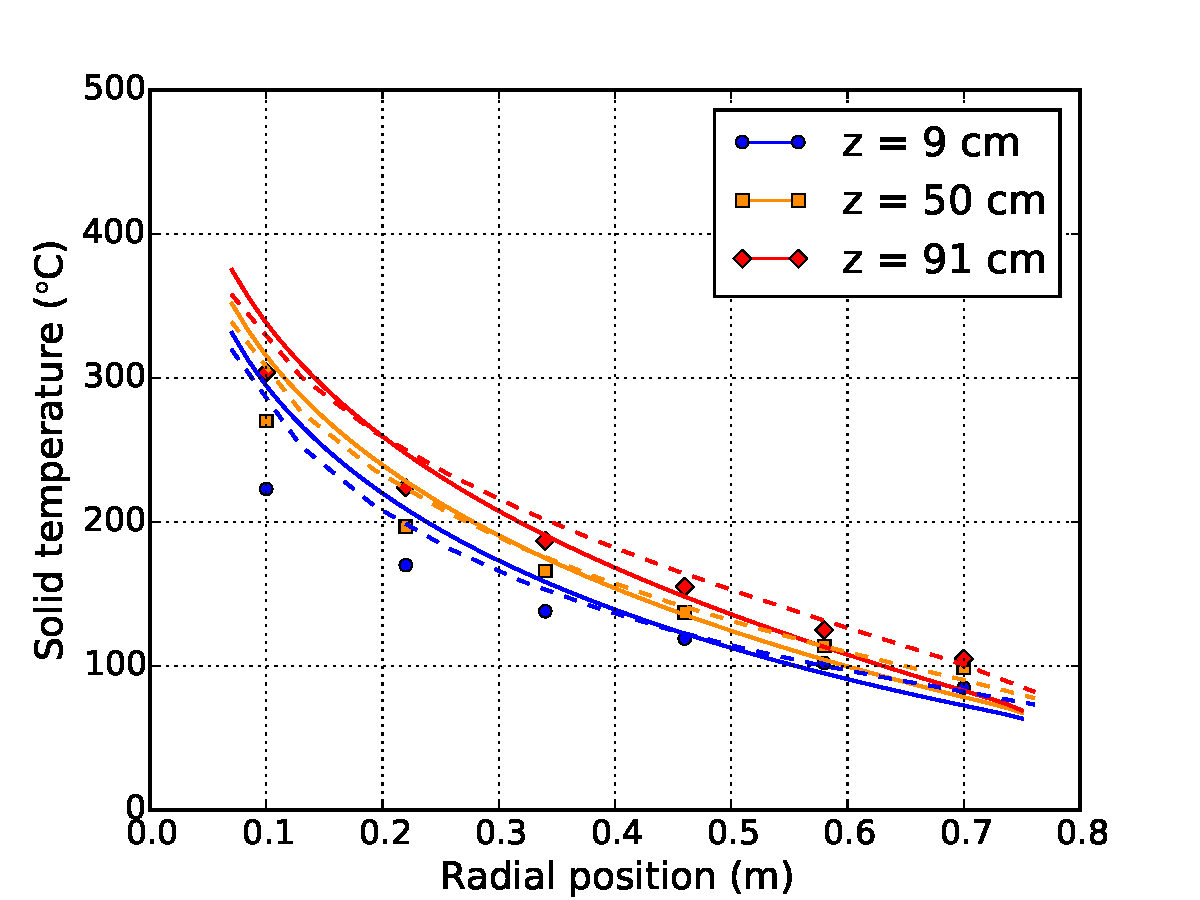
\includegraphics[height=0.75\linewidth]{figs/exp_total_A.pdf}
       \caption{Case A: 5 \si{\kilo\watt} helium}
       \label{fig:helium_longa}
    \end{subfigure}
    \begin{subfigure}{0.5\linewidth}
        \centering
        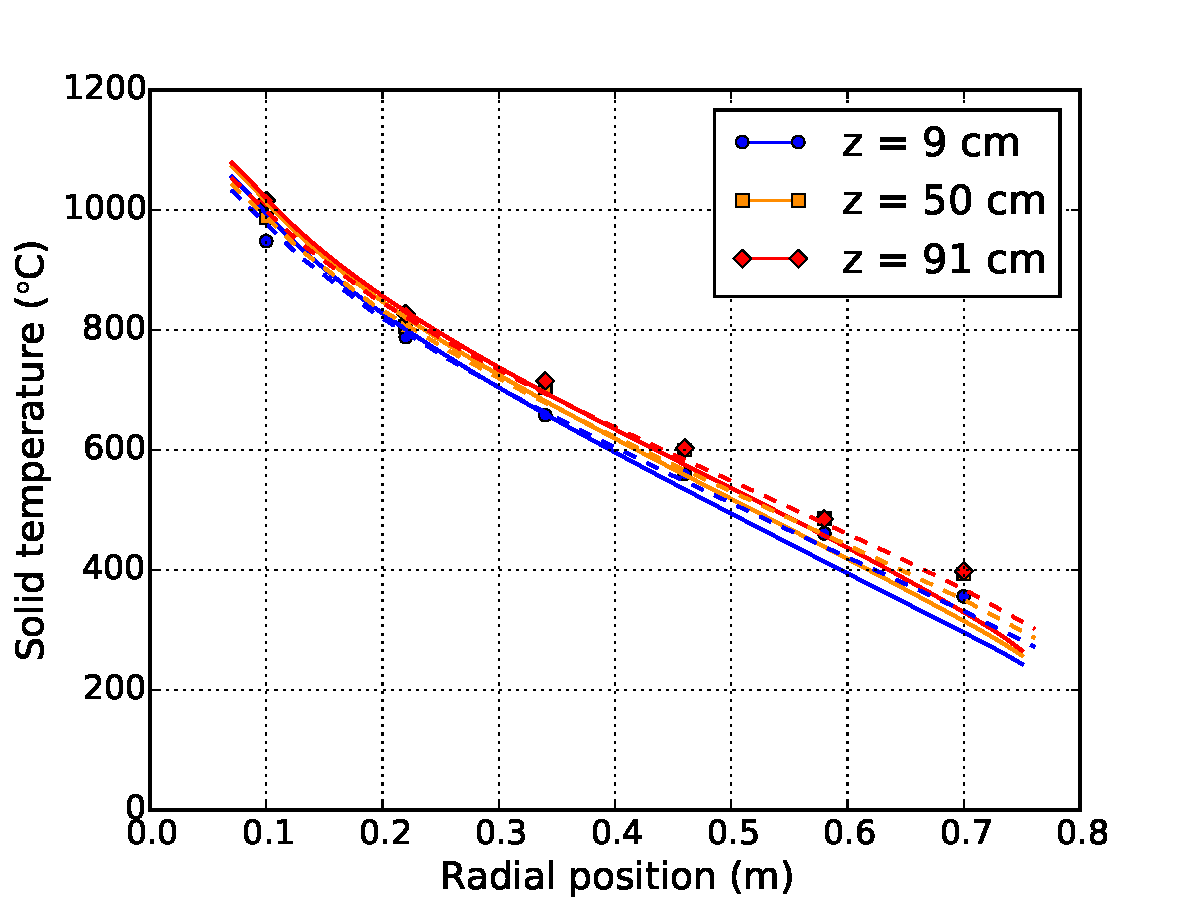
\includegraphics[height=0.75\linewidth]{figs/exp_total_F.pdf}
        \caption{Case B: 35 \si{\kilo\watt} helium}
        \label{fig:helium_longb}
    \end{subfigure}
    \caption{Pronghorn (---) and Flownex (- -) predicted solid temperature at three axial elevations for (a) case A and (b) case B, or a full-length heater with helium and 6 \si{\centi\meter} graphite pebbles.}
    \label{fig:helium_long}
\end{figure}

\begin{figure}[h!]
    \begin{subfigure}{0.5\linewidth}
        \centering
        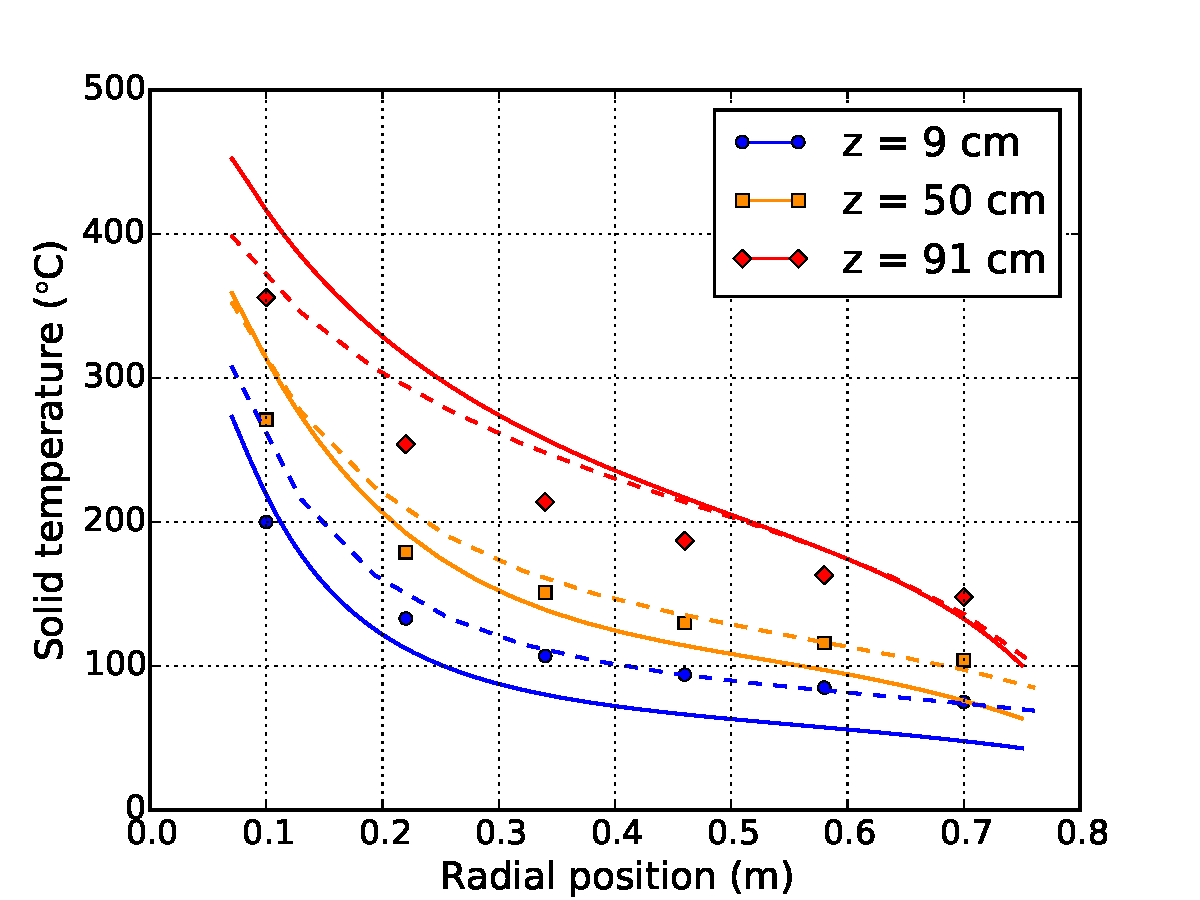
\includegraphics[height=0.75\linewidth]{figs/exp_total_G.pdf}
       \caption{Case C: 5 \si{\kilo\watt} nitrogen}
       \label{fig:nitrogen_longa}
    \end{subfigure}
    \begin{subfigure}{0.5\linewidth}
        \centering
        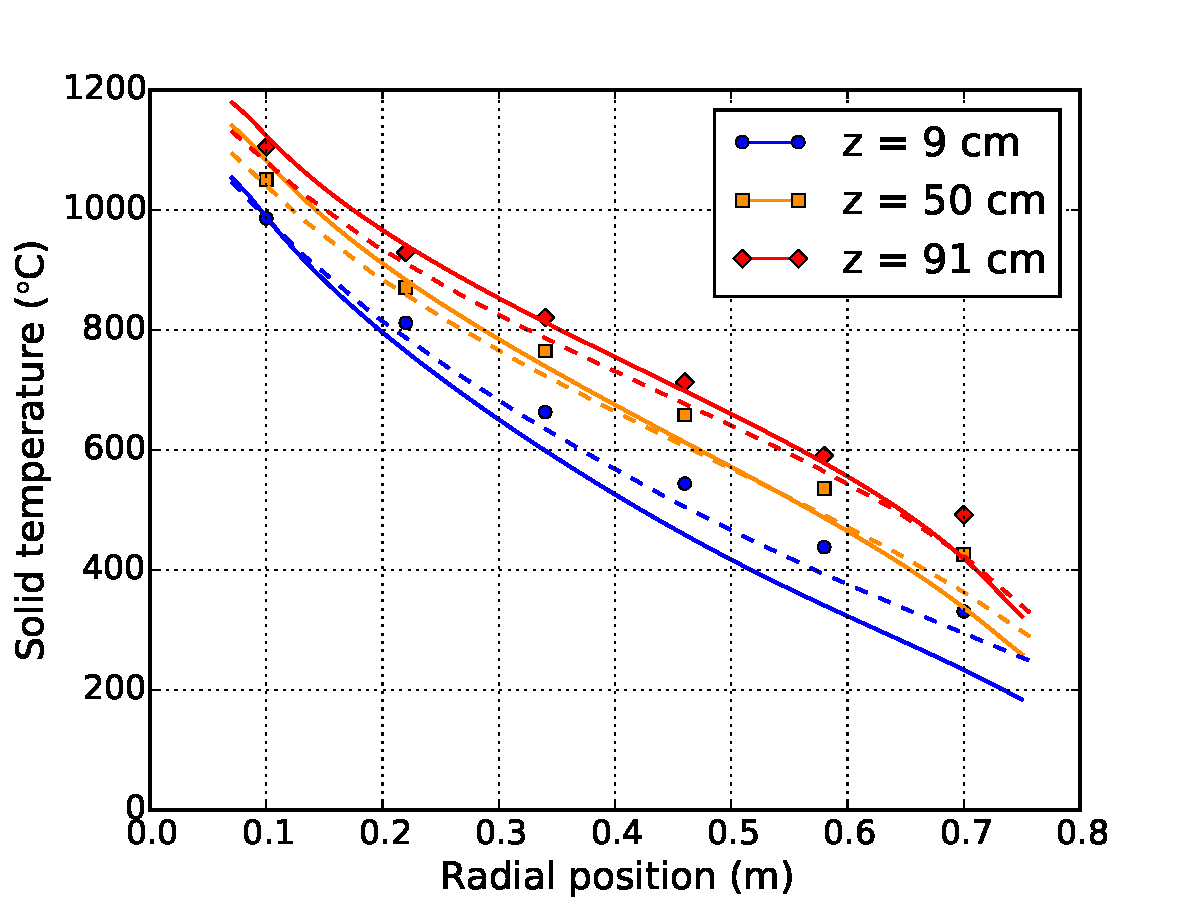
\includegraphics[height=0.75\linewidth]{figs/exp_total_L.pdf}
        \caption{Case D: 35 \si{\kilo\watt} nitrogen}
        \label{fig:nitrogen_longb}
    \end{subfigure}
    \caption{Pronghorn (---) and Flownex (- -) predicted solid temperature at three axial elevations for (a) case C and (b) case D, or a full-length heater with nitrogen and 6 \si{\centi\meter} graphite pebbles.}
    \label{fig:nitrogen_long}
\end{figure}

\begin{figure}[h!]
    \begin{subfigure}{0.5\linewidth}
        \centering
        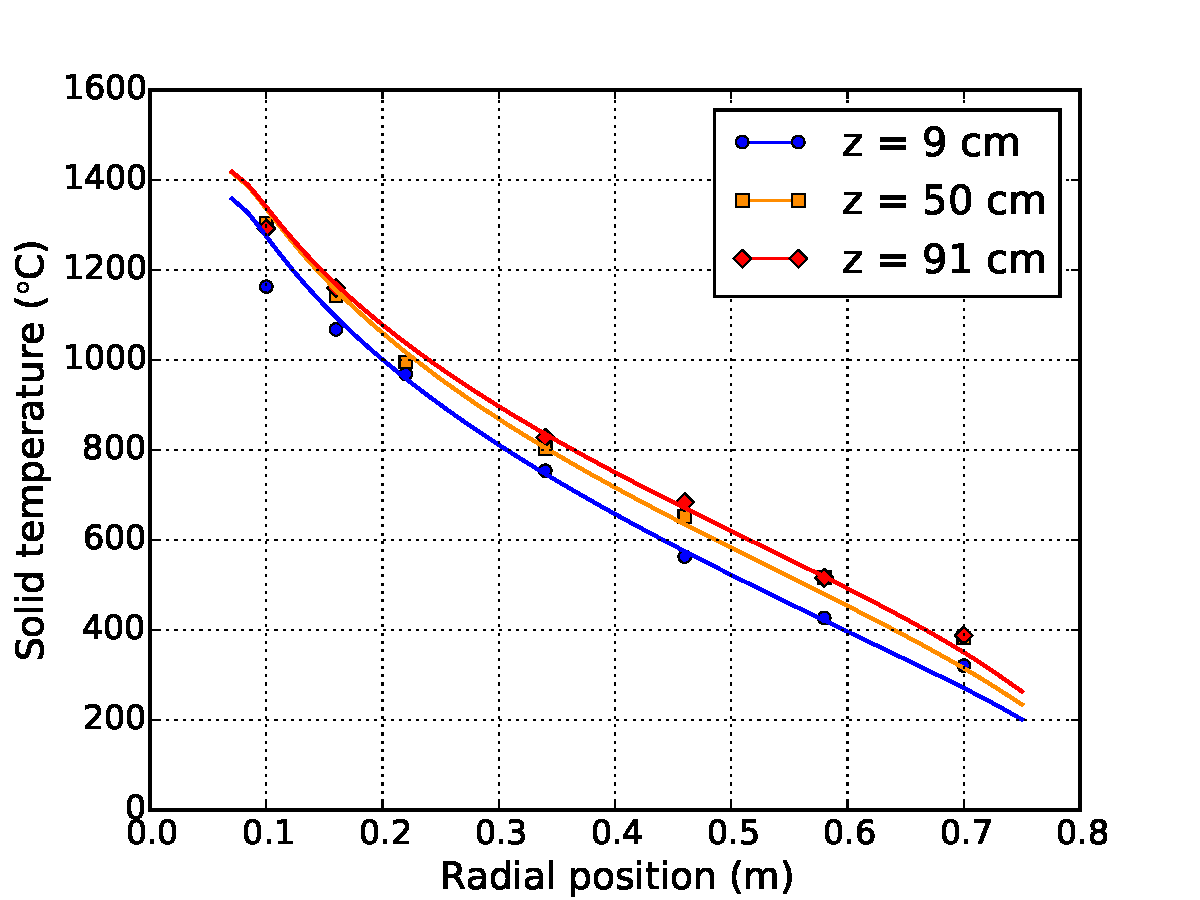
\includegraphics[height=0.75\linewidth]{figs/exp_total_D2.pdf}
       \caption{Case E: 30 \si{\kilo\watt} helium}
    \end{subfigure}
    \begin{subfigure}{0.5\linewidth}
        \centering
        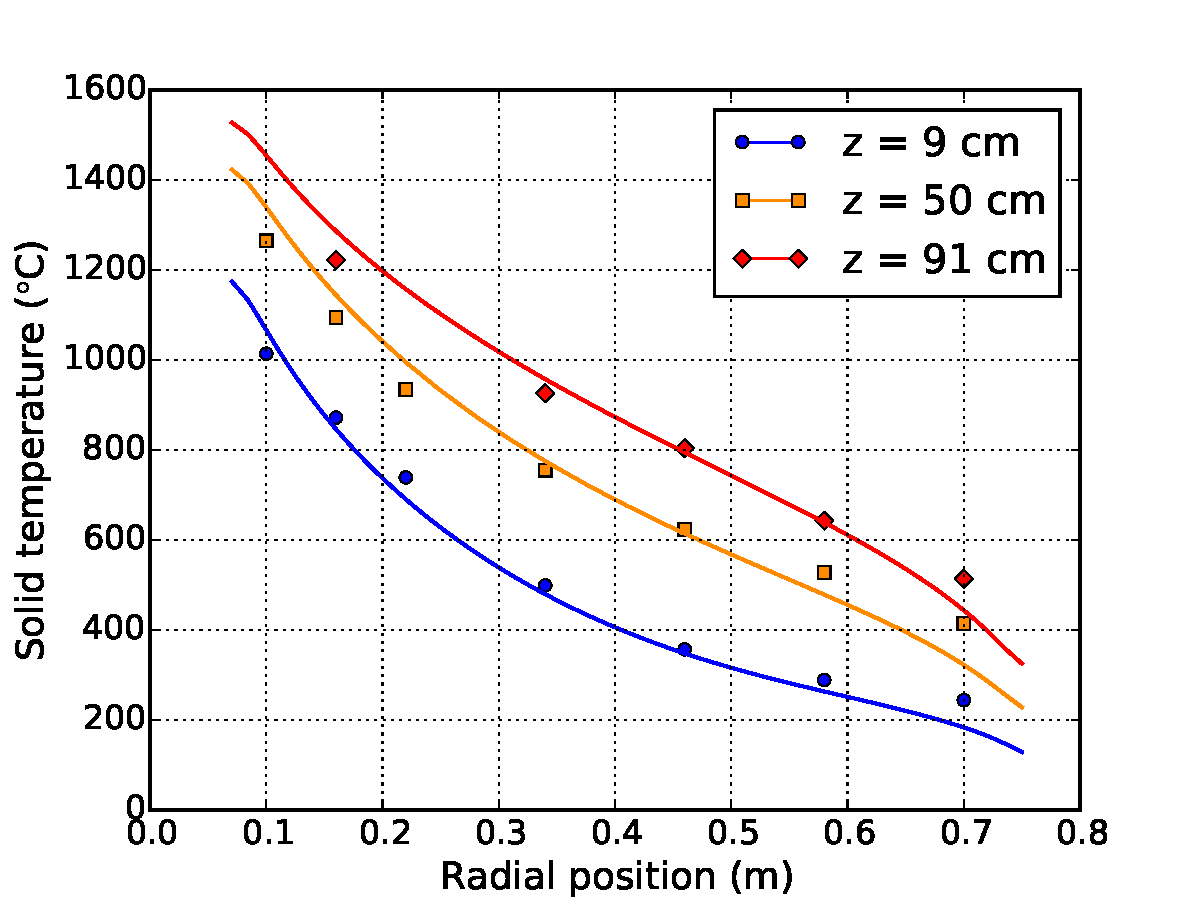
\includegraphics[height=0.75\linewidth]{figs/exp_total_J2.pdf}
        \caption{Case F: 30 \si{\kilo\watt} nitrogen}
    \end{subfigure}
    \caption{Pronghorn (---) predicted solid temperature at three axial elevations for (a) case E and (b) case F, or a full-length heater with helium or nitrogen and 6.5 \si{\centi\meter} aluminum oxide pebbles.}
    \label{fig:long65}
\end{figure}

Fig.\ \ref{fig:bottom} shows Pronghorn, Flownex, and GAMMA solid temperature predictions for a heater power of 20 \si{\kilo\watt} in the bottom half of the bed with 6 \si{\centi\meter} graphite pebbles and helium or nitrogen coolant. Near the heater surface, the temperature distribution is inverted relative to the long central heater cases in Figs. \ref{fig:helium_long} and \ref{fig:nitrogen_long}, being highest at the bottom of the bed. This occurs due to the absence of a heat source in the top of the bed. The lower thermal conductivity of nitrogen results in poorer radial heat transport than in helium, resulting in an opposite temperature trend near the bed periphery compared to helium. All codes show similar trends in Fig.\ \ref{fig:bottom}, but the absolute variation is larger than for the full-length heater results. Pronghorn tends to underpredict temperatures in the higher elevations relative to Flownex and GAMMA. 

\begin{figure}[h!]
    \begin{subfigure}{0.5\linewidth}
        \centering
        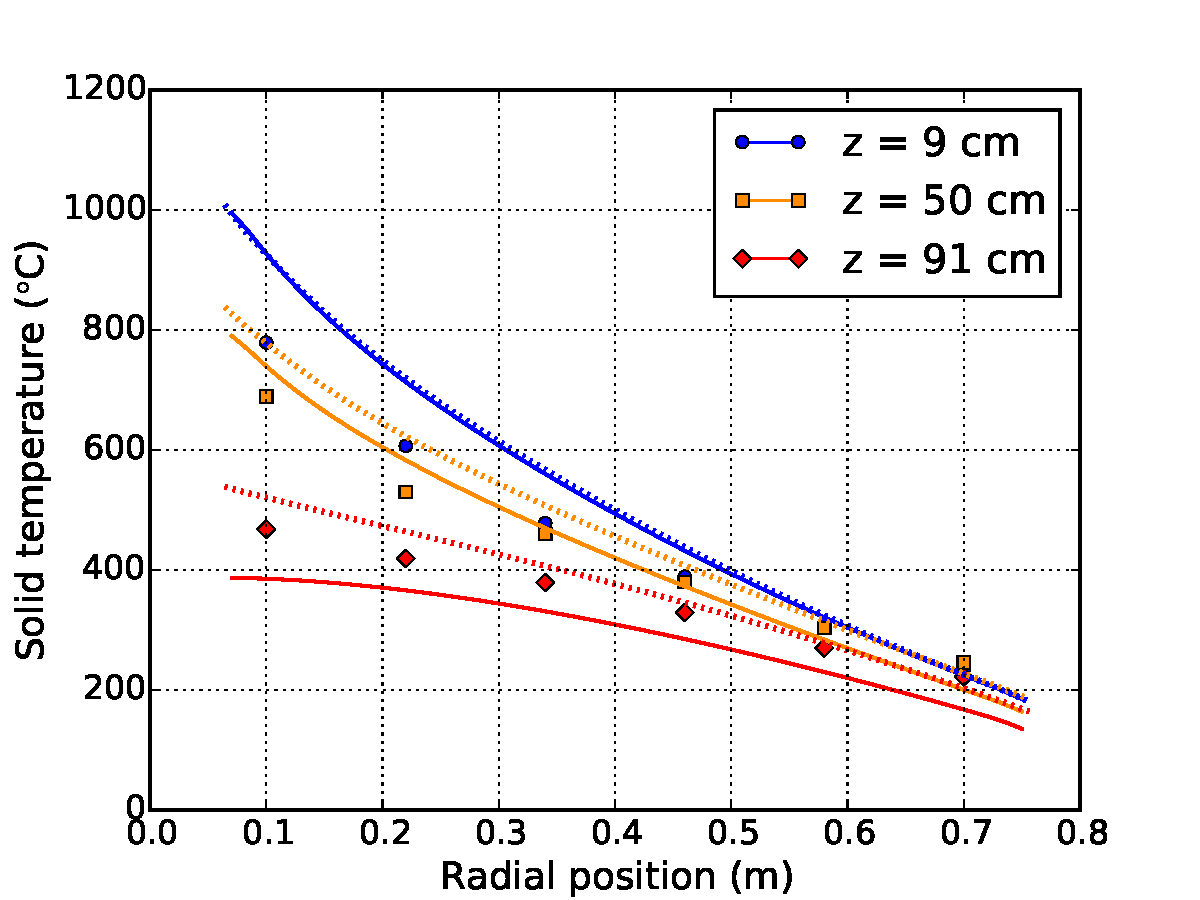
\includegraphics[height=0.75\linewidth]{figs/exp_total_U2.pdf}
       \caption{Case G: 20 \si{\kilo\watt} helium}
    \end{subfigure}
    \begin{subfigure}{0.5\linewidth}
        \centering
        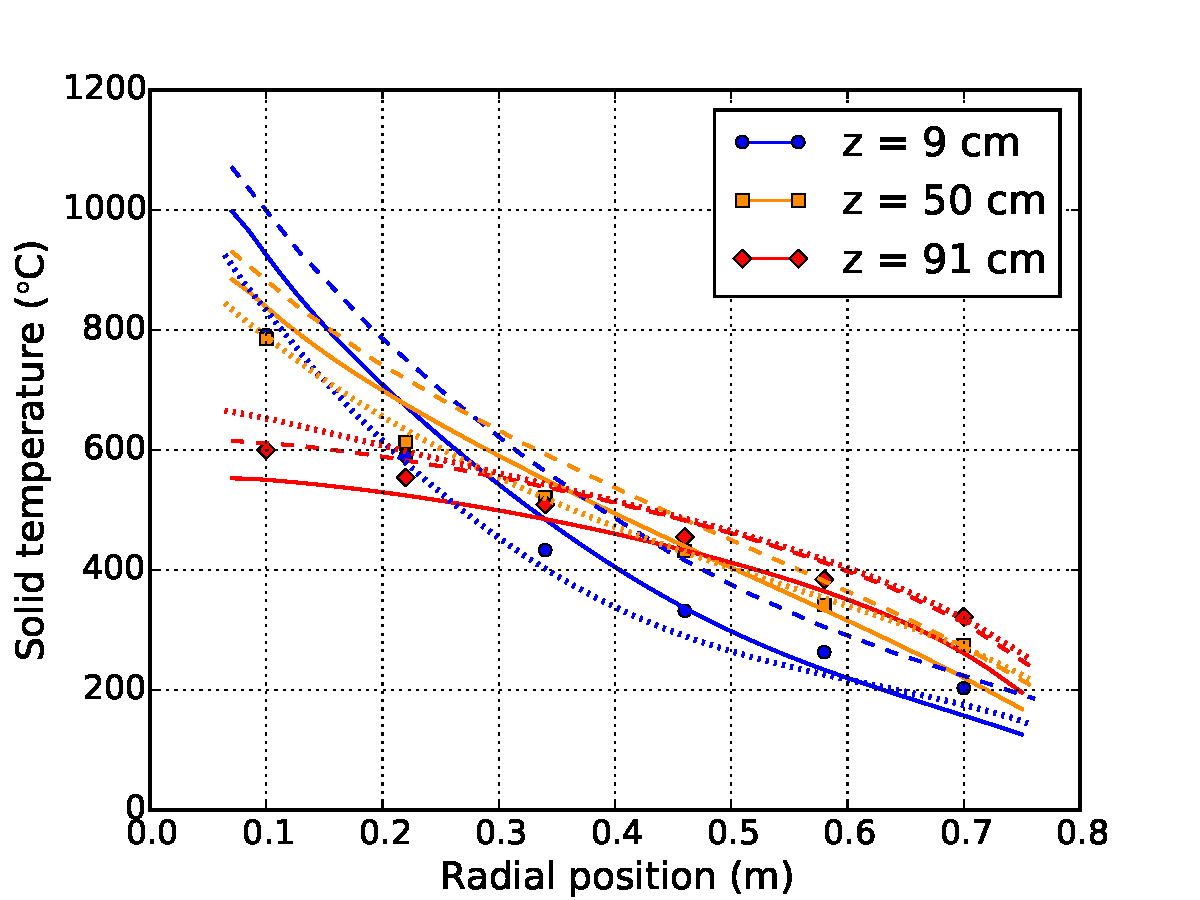
\includegraphics[height=0.75\linewidth]{figs/exp_total_Y2.pdf}
        \caption{Case H: 20 \si{\kilo\watt} nitrogen}
    \end{subfigure}
    \caption{Pronghorn (---), Flownex (- -), and GAMMA (\(\cdots\)) predicted solid temperature at three axial elevations for (a) case G and (b) case H, or a half-length heater in the bottom of the bed and 6 \si{\centi\meter} graphite pebbles.}
    \label{fig:bottom}
\end{figure}

Finally, Fig.\ \ref{fig:plenuma} shows Pronghorn solid temperature predictions for a heater power of 5 \si{\kilo\watt} in the bottom half of the bed and an open plenum in the top third of the bed for 6 \si{\centi\meter} graphite pebbles and nitrogen coolant. Reasonable agreement is obtained with the experimental data, though temperatures are slightly overpredicted near the heater surface at the middle and top elevations. Fig.\ \ref{fig:plenumb} shows predicted fluid temperature with velocity streamlines. The transition from the pebble bed to the open plenum is clearly visible in the velocity streamlines. Fluid re-entering the porous region is pulled towards the high-porosity region near the wall where friction factors are lower. When combined with the significantly reduced friction in the open plenum relative to the bed, this results in primarily radial flow in the plenum.

\begin{figure}[h!]
    \begin{subfigure}{0.5\linewidth}
        \centering
        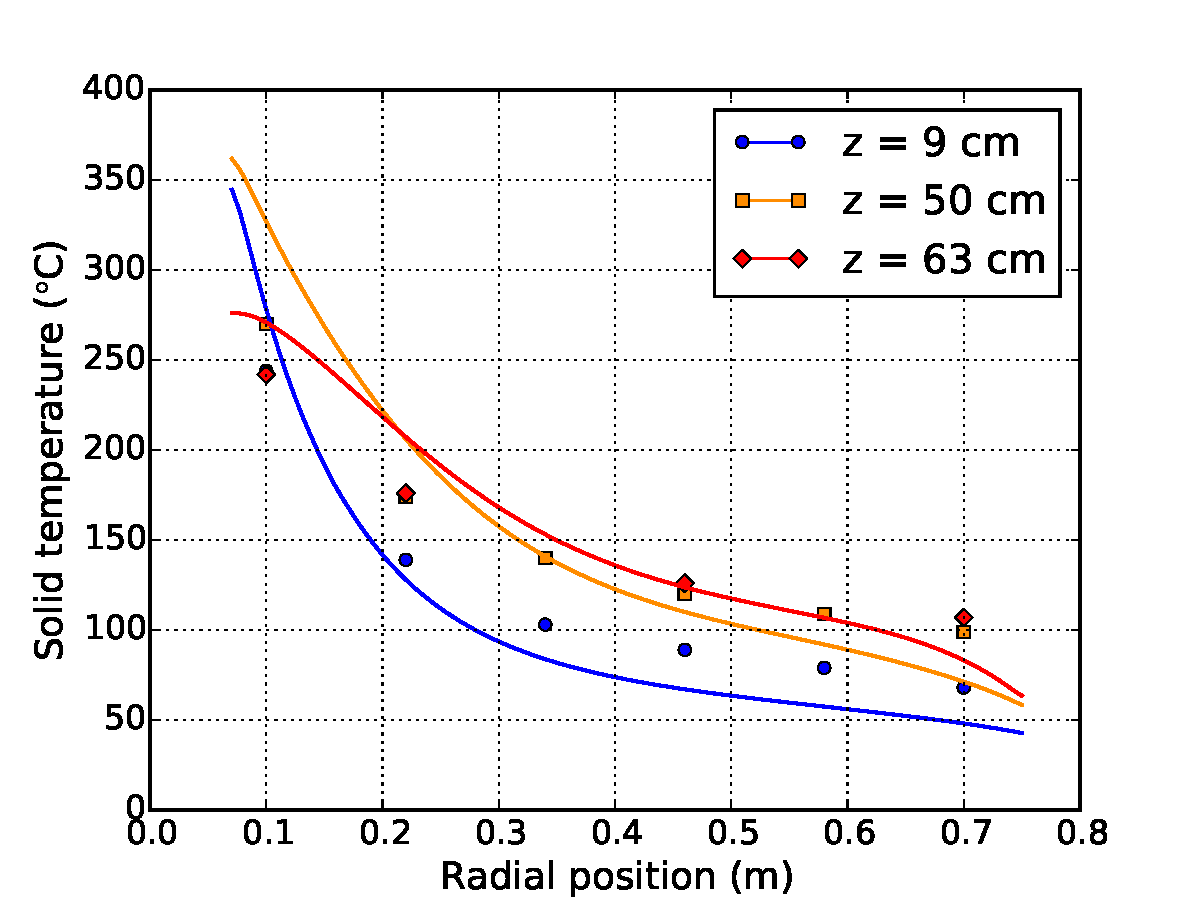
\includegraphics[height=0.75\linewidth]{figs/piecewise_A3.pdf}
       \caption{Solid temperature}
       \label{fig:plenuma}
    \end{subfigure}
        \begin{subfigure}{0.5\linewidth}
        \centering
        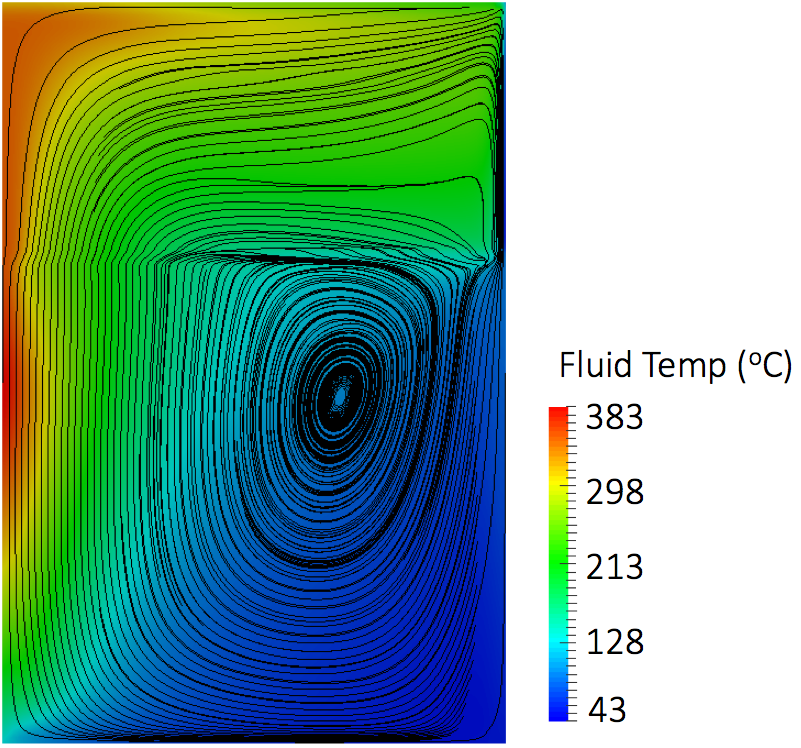
\includegraphics[height=0.75\linewidth]{figs/A3_streamlines.png}
       \caption{Velocity streamlines}
       \label{fig:plenumb}
    \end{subfigure}
    \caption{Pronghorn predicted (a) solid temperature at three axial elevations and (b) fluid temperature with velocity streamlines for case I, or an open plenum and 6 \si{\centi\meter} graphite pebbles.}
    \label{fig:plenum}
\end{figure}

It should be noted that the use of a friction-dominated model in the plenum is not justified as it is in the pebble bed because there is a large mixing region. However, the lack of experimental data for the plenum region precludes directly assessing the accuracy of the plenum velocity and fluid temperature predictions. Additional validation is required for open plenum geometries, though the solution in the bed region agrees reasonably well with experimental data.

\subsection{All Steady-State Axisymmetric Tests}
\label{sec:AllTests}

This section summarizes the results for all 52 steady-state and axisymmetric experiments, with a total of 1292 experimental pebble temperature data points. For simplicity, the plenum test shown at the end of Section \ref{sec:sana_subset} is excluded from the histograms shown here and in Section \ref{sec:sensitivity}. The error relative to the experimental measurements, \(e_\text{num}\) is defined as

\begin{equation}
\label{eq:Error}
e_\text{num}\equiv T_{s}\left(\vec{x}_i\right)-T_{s,\text{exp},i}\ ,
\end{equation}

\noindent where \(T_s\left(\vec{x}_i\right)\) is the predicted solid temperature at position \(\vec{x}_i\) and \(T_{s,\text{exp},i}\) is the experimentally-measured solid temperature at position \(\vec{x}_i\). The maximum error is defined to occur at the data point with error furthest from zero, and may be either positive or negative. 

Fig.\ \ref{fig:histogram} shows a histogram of the error for all 52 cases with the available Flownex and GAMMA data. Significantly more cases were simulated with Pronghorn than with Flownex and GAMMA. To provide a fair comparison of the average error and standard deviation, Table \ref{table:stats} shows the mean, standard deviation \(\sigma\), and maximum error for all 52 cases simulated with Pronghorn, the six cases simulated with Flownex, and the four cases simulated with GAMMA. 

\begin{figure}[h!]
\centering
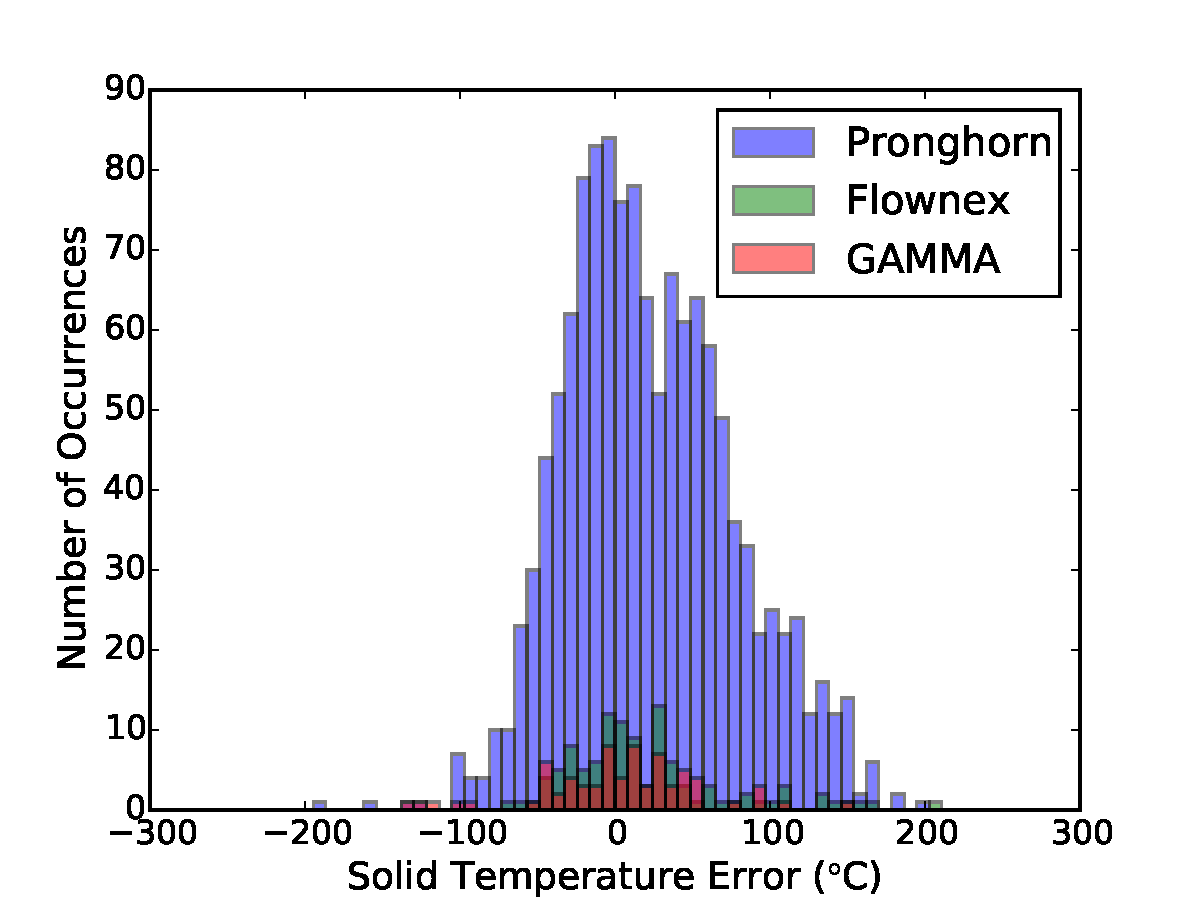
\includegraphics[width=0.6\linewidth]{figs/histogram_abs_error.pdf}
\caption{Histogram of solid temperature error for Pronghorn (52 cases), Flownex (six cases), and GAMMA (four cases).}
\label{fig:histogram}
\end{figure}

In each column, the number of points compared between the three tools are the same. When directly comparing Pronghorn to Flownex and GAMMA, Pronghorn predicts a slightly smaller mean error and lower standard deviation relative to both Flownex and GAMMA. Pronghorn predicts a significantly smaller maximum error for the Flownex cases, but a slightly larger error for the GAMMA cases. Given the cases simulated, the three codes are of comparable accuracy. 

\begin{table}[h!]
\caption{The mean, standard deviation, and maximum solid temperature error for the Flownex cases (A, B, C, D, H, and the 20 \si{\kilo\watt} top half heater with 6 \si{\centi\meter} graphite pebbles and nitrogen); GAMMA cases (G, H, and the 30 \si{\kilo\watt} long heater with 6 \si{\centi\meter} graphite pebbles with helium and nitrogen); and all 52 cases. All units are \si{\celsius}. ``---'' indicates that data is not available.}
\centering
\begin{tabular}{|c |c c c |c c c |c c c|}
\hline\hline
\multicolumn{1}{|c|}{\multirow{2}{*}{Code}} & \multicolumn{3}{c}{Flownex cases (6)} & \multicolumn{3}{c}{GAMMA cases (4)} & \multicolumn{3}{c|}{\color{white}${\rvert^\dagger}^\dagger$\color{black}All cases (52)\color{white}${\rvert^\dagger}^\dagger$\color{black}}\Bstrut\\ \cline{2-10}
 & Mean & \(\sigma\) & Max. & Mean & \(\sigma\) & Max. & Mean & \(\sigma\) & Max.\Tstrut\Bstrut\\
\hline
Flownex & \color{white}-\color{black}19.8 & 51.4 & \color{white}-\color{black}207.0 & --- & --- & --- & --- & --- & ---\Tstrut\\
GAMMA & --- & --- & --- & \color{white}-\color{black}4.3 & 50.9 & 147.5 & --- & --- & ---\\
Pronghorn & \color{white}0\color{black}-7.8 & 47.5 & -155.8 & -1.6 & 48.7 & 148.4 & 22.6 & 54.6 & 198.6\Bstrut\\
\hline
\end{tabular}
\label{table:stats}
\end{table}

It should be noted that the presentation of the error and standard deviation for the SANA cases should not be taken as an indication of the expected accuracy of the macroscale model for all applications. Rather, this condensed presentation is performed to provide a quantitative comparison against Flownex and GAMMA and to provide a rough sense of the accuracy of porous media \gls{th} simulations in friction-dominated flows such as \gls{lofc} decay heat removal.

The standard deviation for all simulation tools is similar, on the order of 50\si{\celsius}. The SANA experiments are a challenging benchmark because of the large thermal gradients near the heater and outer radial wall. Fig.\ \ref{fig:error_location} shows the error in the Pronghorn predictions as a function of distance from the radial and axial walls. Black dots represent individual data points, while larger red dots are the means of the data at each value of the independent variable, either the radial distance or the axial distance. 

The spread, or standard deviation, in the error decreases with distance from radial and axial walls. This is expected because of the isotropic assumptions made in the derivation of porous media closures from bed-averaged data. Additional contributors to near-wall errors include the use of simplified thermal resistance \glspl{bc} and momentum equations that permit slip, the latter of which results in an overprediction of the velocity near the wall and a corresponding overprediction of convective heat transfer and drag. Therefore, the large standard deviation of 50\si{\celsius} can be partially attributed to the significant fraction of experimental data points close to bounding walls. 

\begin{figure}[h!]
    \begin{subfigure}{0.5\linewidth}
        \centering
        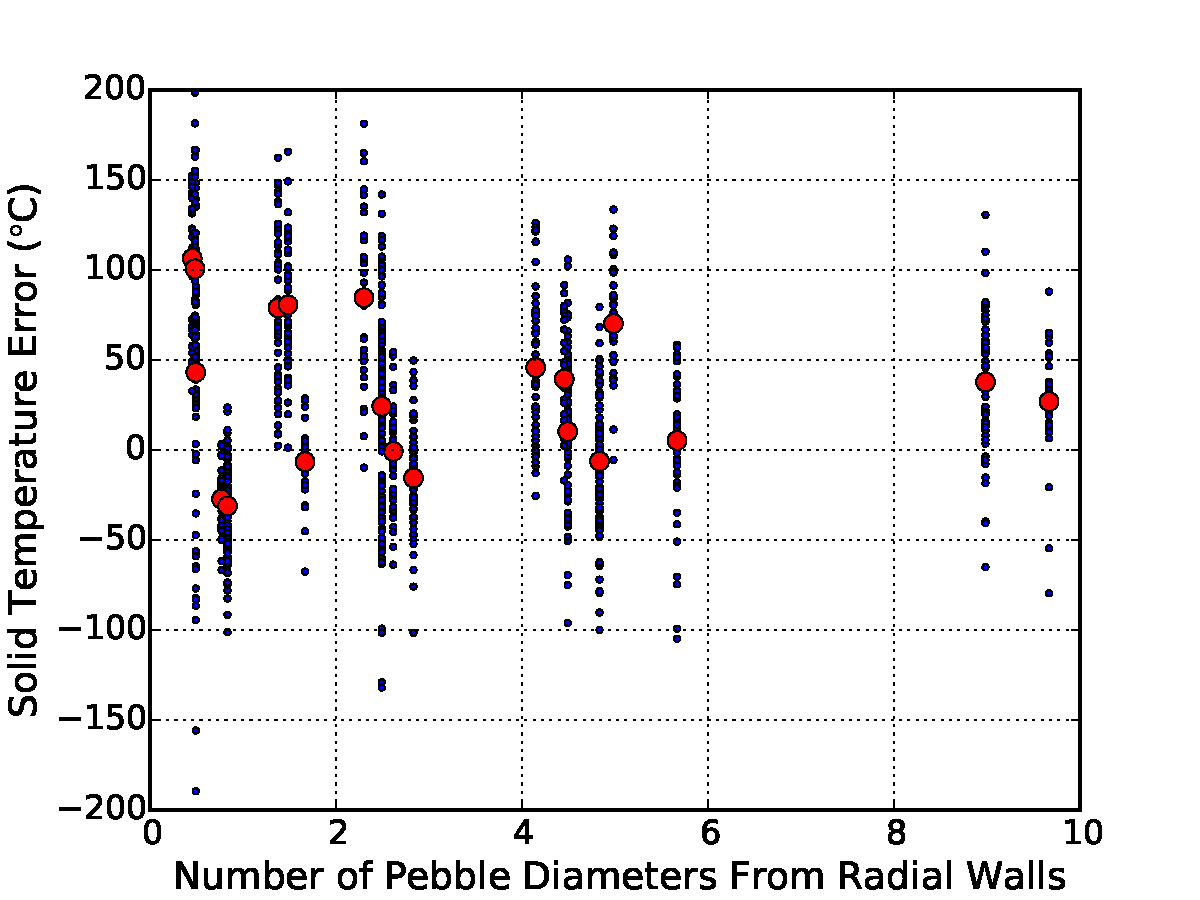
\includegraphics[width=1.0\linewidth]{figs/error_radial.pdf}
       \caption{Error vs. distance from radial wall}
       \label{fig:error_locationa}
    \end{subfigure}
    \begin{subfigure}{0.5\linewidth}
        \centering
        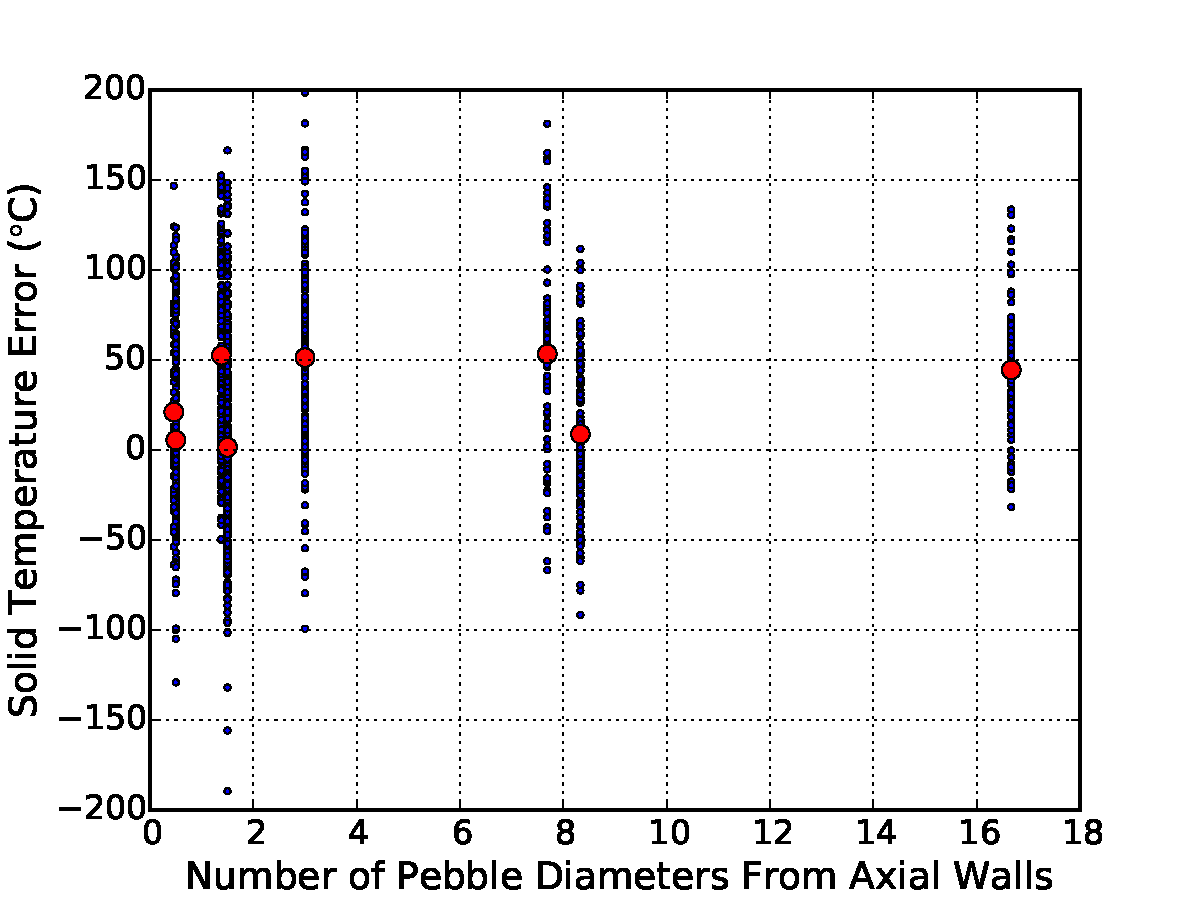
\includegraphics[width=1.0\linewidth]{figs/error_axial.pdf}
        \caption{Error vs. distance from axial wall}
        \label{fig:error_locationb}
    \end{subfigure}
    \caption{Solid temperature error as a function of distance from (a) a radial wall (inner or outer), and (b) an axial wall (lower or upper). Each black dot is one data point. Each red dot is the mean error for the data at each value of the independent variable.}
    \label{fig:error_location}
\end{figure}

Fig.\ \ref{fig:error_locationa} shows that the mean error decreases with distance from the radial walls, while no such trend is clearly visible in Fig.\ \ref{fig:error_locationb} for the mean error as a function of distance from the axial walls. This supports the claim that the SANA experiments are a challenging benchmark due to the very large thermal gradients in the radial direction. No such decrease in average error exists for distances from the axial walls, which are insulated to the extent that thermal boundary effects are less significant but are still characterized by slip effects and anisotropic momentum and heat transfer. This suggests that 1)~the average error in Pronghorn simulations will be lower for systems with less significant thermal boundary layers; and 2)~more sophisticated heat flux \glspl{bc} can potentially reduce mean error in the near-wall regions. 

On average, Pronghorn overpredicts the solid temperature by 22.6\si{\celsius}. In addition to the identified near-wall error contributions of isotropic closures, slip, and simplified resistance \glspl{bc}, additional modeling approximations that may have affected the accuracy of the simulations include the constant vessel surface convection coefficient and emissivity and the constant pebble emissivity, elastic modulus, and Poisson ratio. In all cases shown in Section \ref{sec:baseline}, temperatures are generally overpredicted near the heater surface. This may indicate that the closures used for \(\kappa_s\) underpredict the effective thermal conductivity in this region or that the pebble emissivity is too low. Pebble emissivities of 0.9 and 0.85 have been used in other simulations of \glspl{pbr} \cite{tecdoc1163,tecdoc1694}. Therefore, a higher emissivity is not without precedent, but an emissivity of 0.8 is used for easier comparison to Flownex and GAMMA. 

Additional insight can be obtained when considering the error for different subsets of the experiments as summarized in Table \ref{table:subcases}. On average, Pronghorn predicts the helium cases with 16.6\si{\celsius} lower standard deviation than the nitrogen cases. The maximum error for the nitrogen cases is 31.9\si{\celsius} higher than for the helium cases. The greater convective transport in nitrogen is more difficult to capture with the friction-dominated model. 

\begin{table}[h!]
\caption{The mean, standard deviation, and maximum error for different subsets of the 52 steady-state and axisymmetric SANA cases.}
\centering
\begin{tabular}{|r |c |c c c |}
\hline\hline
\multicolumn{1}{|c|}{Subset Description} & \# Cases & Mean (\si{\celsius}) & \(\sigma\) (\si{\celsius}) & Max. (\si{\celsius})\Tstrut\Bstrut\\
\hline
\textbf{All cases} & \textbf{52} & \textbf{22.6} & \textbf{54.6} & \textbf{\color{white}-\color{black}198.6}\Tstrut\\
Helium coolant & 26 & 20.5 & 45.8 & \color{white}-\color{black}166.7\\
Nitrogen coolant & 26 & 24.8 & 62.4 & \color{white}-\color{black}198.6\\
3 \si{\centi\meter} matrix graphite pebbles & 12 & 44.2 & 48.7 & \color{white}-\color{black}198.6\\
6 \si{\centi\meter} electric graphite pebbles & 28 & \color{white}0\color{black}2.0 & 48.4 & -189.6\\
6.5 \si{\centi\meter} aluminum oxide pebbles & 12 & 45.8 & 55.8 & \color{white}-\color{black}181.3\\
Full-length heater & 36 & 30.5 & 52.7 & \color{white}-\color{black}198.6\\
Partial-length heater & 16 & \color{white}0\color{black}3.9 & 54.7 & -189.6\Bstrut\\
\hline
\end{tabular}
\label{table:subcases}
\end{table}

Pronghorn predicts temperatures with the aluminum oxide pebbles with a standard deviation approximately 7.3\si{\celsius} higher than the two types of graphite pebbles. This may be attributed to the use of graphite emissivity, Young's modulus, and Poisson ratio for the aluminum oxide pebbles due to a lack of aluminum oxide data. 

The 6 \si{\centi\meter} graphite pebble cases are predicted with remarkably lower mean error than the other two types of pebbles. While this may be partially attributable to the fact that partial-length heater cases were only performed with the 6 \si{\centi\meter} graphite pebbles, this lower error may be related to the use of the \gls{kta} correlations for drag and heat transfer, which were developed based on experiments using 6 \si{\centi\meter} graphite pebbles. Lower errors for the 3 \si{\centi\meter} matrix graphite and 6.5 \si{\centi\meter} aluminum oxide pebbles might be obtained if using closures based on those specific pebble designs. Finally, a margin of 1\% in temperature, 2 \si{\centi\meter} in axial position, and 1 \si{\centi\meter} in radial position are the levels of uncertainty in the experimental measurements themselves \cite{becker2003}.

Overall, good agreement is obtained with both Flownex and GAMMA. Visual comparisons against THERMIX, TINTE, and TRIO-EF results available in the literature \cite{tecdoc1163} show good agreement with Pronghorn. Differences between Pronghorn, Flownex, and GAMMA exist because of the use of different closures, equation models, and \glspl{bc}. For example, neither Flownex nor GAMMA consider an axial dependence in the porosity, while Pronghorn considers a 2-D \(r\)-\(z\) dependence. Flownex and GAMMA include a viscous stress term in the conservation of momentum equation, while Pronghorn permits slip. Flownex uses a constraint-style equation to represent heat transfer between pebbles, while Pronghorn and GAMMA combine the solid effective heat transfer term with the conservation of solid energy equation. Different vessel surface convection coefficients are used in all three applications.

Significant development efforts in all three applications are required to fully disentangle these simultaneous effects to identify the most significant contributors to the different temperature predictions. Simulations of a small subset of the SANA experiments with the compressible Navier-Stokes macroscale model suggest that temperatures may differ by up to 20 to 30\si{\celsius} in some regions of the bed, though not always in the direction of lower error \cite{schunert_phr}. A rigorous quantification of the effect of macroscale model differences between Pronghorn, Flownex, and GAMMA is an area of future work. 

\section{Sensitivity to Macroscale Closures}
\label{sec:sensitivity}

This section explores the sensitivity of pebble temperature to particular closures for porosity, the near-wall treatment for the solid effective thermal conductivity, interphase heat transfer and drag, and thermal dispersion. The geometric representation and \glspl{bc} described in Section \ref{sec:model} are unchanged.

Table \ref{table:stats_location} shows the mean, standard deviation, and maximum error for the baseline Pronghorn model in comparison to various closure modifications. The data in each row was obtained by simulating all 52 steady-state and axisymmetric cases with a single isolated change in macroscale closures from the baseline model described in Section \ref{sec:model}. For example, the entry labeled ``constant porosity'' represents simulation predictions with the porosity closure used in the baseline model replaced by the constant porosity model in Eq. \eqref{eq:ConstantEps} with all other closures fixed. ``Near-wall scaling \(\kappa_s\)'' represents predictions with a \(0.5\) multiplier on \(\kappa_\text{radiation}\) in the near-wall region instead of the Tsotsas correlation in Eq. \eqref{eq:Tsotsas}. ``Ergun \(W\)'' represents predictions with the Ergun interphase friction factor in Eq. \eqref{eq:Ergun} instead of the \gls{kta} correlation in Eq. \eqref{eq:W_KTA}. ``Gnielinski \(\alpha\)'' represents predictions with the Gnielinski interphase convective heat transfer coefficient in Eq. \eqref{eq:GnielinskiPebblebed} instead of the \gls{kta} correlation in Eq. \eqref{eq:KTA}. ``With dispersion'' represents predictions with the linear Peclet dispersion model in Eq. \eqref{eq:LinearPecletKappaFluid} instead of the zero-dispersion model in Eq. \eqref{eq:KappaFluidBasic}.

To quantify the significance of the lack of complete experimental facility information, simulations are also performed for two different constant values of the vessel convection coefficient and for two different values of the pebble emissivity. Results are presented in terms of the thermocouple locations within the bed to illustrate how the error varies as a function of position. The near-wall region is defined to occur within a half pebble diameter of the walls, while the bulk region constitutes all other points. 459 points lie in the near-wall region, while the remaining 833 are in the bulk.

\begin{table}[h!]
\caption{The mean, standard deviation, and maximum solid temperature error for all 52 cases simulated with Pronghorn as a function of location within the bed for various closure modifications to the baseline model described in Section \ref{sec:model}. All units are \si{\celsius}.}
\centering
\centerline{
\begin{tabular}{|r |c c c |c c c |c c c|}
\hline\hline
\multicolumn{1}{|c|}{\multirow{2}{*}{Model}} & \multicolumn{3}{c}{\color{white}${\rvert^\dagger}^\dagger$\color{black}All\color{white}${\rvert^\dagger}^\dagger$\color{black}} & \multicolumn{3}{c}{Near-Wall} & \multicolumn{3}{c|}{Bulk}\Bstrut\\ \cline{2-10}
 & Mean & \(\sigma\) & Max. & Mean & \(\sigma\) & Max. & Mean & \(\sigma\) & Max.\Tstrut\Bstrut\\
\hline
\textbf{Baseline} & \textbf{22.6} & \textbf{54.6} & \textbf{\color{white}-\color{black}198.6} & \textbf{29.3} & \textbf{60.5} & \textbf{\color{white}-\color{black}198.6} & \textbf{18.9} & \textbf{50.7} & \textbf{181.3}\Tstrut\\
Constant \(\epsilon\) & 34.2 & 66.0 & \color{white}-\color{black}280.1 & 42.1 & 74.4 & \color{white}-\color{black}280.1 & 29.8 & 60.4 & 250.4\\
Near-wall scaling \(\kappa_s\) & 35.5 & 52.0 & \color{white}-\color{black}197.3 & 41.3 & 58.5 & \color{white}-\color{black}197.3 & 32.3 & 47.8 & 191.1\\
Ergun \(W\) & 21.1 & 54.4 & \color{white}-\color{black}211.6 & 27.2 & 59.7 & -197.8 & 17.7 & 50.9 & 211.6\\
Gnielinski \(\alpha\) & 22.0 & 54.9 & \color{white}-\color{black}211.1 & 28.2 & 60.3 & -196.3 & 18.6 & 51.4 & 211.1\\
With dispersion & 21.5 & 54.2 & \color{white}-\color{black}208.1 & 27.5 & 59.6 & \color{white}-\color{black}194.1 & 18.1 & 50.7 & 208.1\Bstrut\\
\hline
\(h_c=10\) \si{\watt\per\square\meter\per\kelvin} & 36.1 & 51.3 & \color{white}-\color{black}218.0 & 41.4 & 57.0 & \color{white}-\color{black}206.8 & 33.2 & 47.6 & 218.0\Tstrut\\
\(h_c=20\) \si{\watt\per\square\meter\per\kelvin} & 11.6 & 57.8 & -215.3 & 18.5 & 63.1 & -215.3 & \color{white}0\color{black}7.8 & 54.3 & 203.6\Bstrut\\
\hline
\(\varepsilon=0.7\) & 35.5 & 63.6 & \color{white}-\color{black}221.4 & 45.0 & 70.7 & \color{white}-\color{black}221.4 & 30.3 & 58.7 & 195.0\Tstrut\\
\(\varepsilon=0.9\) & \color{white}0\color{black}9.5 & 48.8 & -179.5 & 13.7 & 53.9 & -179.5 & \color{white}0\color{black}7.2 & 45.7 & 167.3\Bstrut\\
\hline
\end{tabular}
}
\label{table:stats_location}
\end{table}

For all models in Table \ref{table:stats_location}, the mean error and standard deviation are both approximately 10\si{\celsius} higher in the near-wall region than in the bulk. This is expected due to the use of isotropic macroscale closures and the use of slip \glspl{bc}, and is in line with the dependence shown in Fig.\ \ref{fig:error_location}. Interestingly, the location of the maximum error is not wholly dominated by the near-wall region; of the 10 models considered, the highest error occurs in the bulk region for four models.

Less than 2\si{\celsius} difference in both the mean and standard deviation are observed when varying the drag, interphase heat transfer, and thermal dispersion models. This relative average insensitivity to the drag and heat transfer correlation agrees with results observed by others \cite{becker}. However, the maximum error for the Ergun drag model, the Gnielinski convective heat transfer model, and the linear Peclet thermal dispersion model result in 26.8 to 30.3\si{\celsius} higher maximum error in the bulk region, but little absolute change in the near-wall region. 

The solid temperature is sensitive to both the porosity model and the near-wall effective solid thermal conductivity treatment. A constant porosity on average results in a 11.6\si{\celsius} higher error and a 11.4\si{\celsius} higher standard deviation than a 2-D porosity. The maximum error in the near-wall and bulk regions increases by 81.5\si{\celsius} and 69.1\si{\celsius}, respectively. A simple scaling factor applied to the effective solid thermal conductivity in the near-wall region results in a 12.9\si{\celsius} higher error, but a 2.6\si{\celsius} lower standard deviation, than the use of a different \(\kappa_\text{radiation}\) correlation. The maximum error in the near-wall region is relatively unaffected, while the maximum error in the bulk region increases by 9.8\si{\celsius}.

While a constant porosity only differs from the 2-D \(r\)-\(z\) porosity in the near-wall region, and the wall treatment for solid effective thermal conductivity is only applied in the near-wall region, it is important to note that the use of these different closures affects the accuracy in all regions of the bed. Additional investigations are required to determine how these conclusions extend to geometries with larger bed to pebble diameter ratios. 

The solid temperature is also sensitive to the vessel convection coefficient and pebble emissivity. A range of 24.5\si{\celsius} in mean error and 6.5\si{\celsius} in standard deviation is observed depending on the selection of \(h\), while a range of 26.0\si{\celsius} in mean error and 14.8\si{\celsius} in standard deviation is observed depending on the selection of \(\varepsilon\). For all the variations in closure parameters, increasing the pebble emissivity from 0.8 to 0.9 is the only change that simultaneously results in a lower mean error, a smaller standard deviation, and a lower maximum error relative to the baseline model. This strong dependence on emissivity has been observed elsewhere, and motivates complete characterization of pebble material properties \cite{tecdoc1163}. Some error and spread in the Pronghorn simulations must therefore be attributed to a lack of complete experimental and material details in the benchmark specifications.

\section{Summary and Conclusions}
\label{sec:5_summary}

Essential to the development of any new simulation tool is the establishment of a strong validation base. This section demonstrated validation of the friction-dominated macroscale model and its numerical implementation in Pronghorn with the SANA experiments, a scaled experiment modeling depressurized natural convection decay heat removal. Using a single baseline set of closures, Pronghorn on average overpredicts solid temperature by 22.6\si{\celsius} with a standard deviation of 54.6\si{\celsius}. A code-to-code comparison with Flownex and GAMMA shows similar accuracy, with the additional advantages of 3-D unstructured meshing and comprehensive multiphysics coupling to \gls{moose} applications. 
% TODO: Rachel wants something about runtimes

The standard deviation decreases with distance from radial and axial walls, while the error only decreases with distance from radial walls. These observations highlight the need for anisotropic drag and heat transfer closures for near-wall regions, which are all but absent from the porous media literature. The primarily radial temperature gradient in the SANA facility also suggests that more accurate predictions can be achieved with improved isotropic closures such as heat flux \glspl{bc} and near-wall corrections to the effective solid thermal conductivity. 

Future computational and physical experiments must consider the near-wall region as distinct from the bulk region. Multiscale coupling to high-resolution \gls{cfd} or the incorporation of new experimentally-derived closures has the potential to reduce the standard deviation in near-wall regions and consequently achieve more precise predictions of \gls{pbr} \gls{th} to allow reactor design with smaller thermal margins and improved economic viability. The SANA experiments are particularly well-suited for a multiscale demonstration due to the relatively small vessel size and the high number of measurements taken within \(d_p/2\) distance from walls.

The standard deviation and maximum error are 16.6\si{\celsius} higher and 31.9\si{\celsius} higher, respectively, for the experiments with nitrogen coolant. The greater convective transport in nitrogen than in helium is more difficult to capture with the friction-dominated model. Future work will repeat the SANA experiments with the compressible Navier-Stokes model to determine the improvement in accuracy when considering momentum advection.

Interestingly, the error is about 40\si{\celsius} lower for the experiments with 6 \si{\centi\meter} diameter graphite pebbles than for the other two pebble types. While this may be partially attributable to the absence of partial-length heater tests with other pebbles, this lower error may also be due to the use of macroscale heat transfer and drag closures obtained specifically from experiments with 6 \si{\centi\meter} diameter graphite pebbles \cite{KTA,KTAhtc}. Further, the higher error associated with the aluminum oxide pebble experiments and the sensitivity to the vessel convection coefficient and pebble emissivity show that a potentially large systematic error term is present resulting from incomplete experimental characterization.

Statistical analysis shows that the interphase drag, heat transfer, and thermal dispersion models are, on average, of little significance to solid temperature, though errors in the bulk region of the bed increased by up to 30.3\si{\celsius} when using different closures. The solid temperature is sensitive to the models used for porosity and the near-wall treatment of the solid effective thermal conductivity in the entirety of the bed. The highest single increase in error of 81.5\si{\celsius} was observed when switching from a 2-D porosity distribution to a constant distribution. Similar sensitivity studies should be repeated for more systems to generalize these conclusions as a function of power density, bed size, and other characteristic scales.
